\documentclass[a4paper,oneside,12pt]{amsart}

%\usepackage[spanish, activeacute]{babel}
\usepackage[utf8]{inputenc}
%\usepackage[latin1]{inputenc}
\usepackage{latexsym}
\usepackage{multicol}
\usepackage{enumerate}
\usepackage[heightrounded]{geometry}
\geometry{top=2cm,bottom=2cm,left=2cm,right=2cm}
\usepackage{graphicx}
\usepackage{tikz}
\usepackage{amssymb}
\usepackage{tikz-network}

\DeclareMathOperator{\cond}{cond}
\DeclareMathOperator{\Id}{Id}
\DeclareMathOperator{\re}{Re}
%\DeclareMathOperator{\im}{Im}
\newcommand{\I}{\mathbb{I}}
\newcommand{\R}{\mathbb{R}}
\newcommand{\Q}{\mathbb{Q}}
\newcommand{\C}{\mathbb{C}}
\newcommand{\Z}{\mathbb{Z}}
\newcommand{\N}{\mathbb{N}}
\DeclareMathOperator{\im}{Im}

\newcommand{\nombremateria}
{Investigaci\'on Operativa}
\newcommand{\nombrecuatrimestre}
    {Segundo cuatrimestre de 2021}
\newcommand{\numeroparcial}
    { Tercer Parcial }
\newcommand{\fecha}
    {19 de Noviembre de 2021}
\newcommand{\numerotema}
    {\bf 1}

%\oddsidemargin -1cm \evensidemargin -1cm \textwidth 17.5cm
%topmargin 1.2cm \textheight 25cm
%\setlength{\textheight}{25cm}

\def \ds{\displaystyle}
\newtheorem{quest}{Ejercicio}
\thispagestyle{empty}

\begin{document}

\hfill \hfill
\begin{tabular}[c]{|c|c|c|c|c|c|}
\hline 
1 & 2 & 3 & 4 & 5 & Calificaci\'on \\ \hline \hline
\hspace{1.2 cm} & \hspace{1.2 cm} & \hspace{1.2 cm} & \hspace{1.2 cm} & \hspace{1.2 cm} &\hspace{1.5 cm} \\
\hspace{1.2 cm} & \hspace{1.2 cm} & \hspace{1.2 cm} & \hspace{1.2 cm} & \hspace{1.2 cm} &\hspace{1.5 cm} \\ \hline

\end{tabular}

\vspace{-1cm}

\noindent Nombre y apellido:

\vspace{0.2cm}

\noindent Número de libreta:

\noindent \hrulefill 

\smallskip
\renewcommand{\baselinestretch}{1.1}

\begin{center}
	\large \textbf{\nombremateria} 
	
	\numeroparcial -- \fecha
\end{center}

\vspace{.6cm}
\renewcommand{\theenumi}{\textbf{\arabic{enumi}}}

%%% EMPIEZA EL EJERCICIO 1 %%%

\begin{quest} 
    Dado un grafo conexo $G=(V,E)$, sea $V'\subsetneq V$ y sea $e$ una arista de peso mínimo que conecta a $V'$ con $V-V'$, entonces existe un árbol generador mínimo de $G$ que contiene a $e$. 

\end{quest}

%%% TERMINA EL EJERCICIO 1 %%%

%%% EMPIEZA EL EJERCICIO 2 %%%

\begin{quest} \hfill
\begin{enumerate} 
    \item Dado $G=(V,E)$ un grafo conexo $(m-1)$-regular tal que $|V|=p\cdot m$ con $p\geq 2$, probar que el tamaño del conjunto independiente máximo es, por lo menos, $p+1$.
    \item Un bloque de un grafo es un subgrafo conexo maximal sin puntos de corte. Sea \newline {$G=(V, E)$} conexo y euleriano, probar que todo bloque de $G$ es euleriano.
    % \item Se tiene la siguiente red $G$ por la que pasa cierto flujo $f$. La red cuenta con dos fuentes $s_1, s_2$ y un sumidero $t$. Plantear el problema como un problema al cual pueda aplicársele un algoritmo de tipo Ford-Fulkerson para hallar flujo máximo y utilizar dicho algoritmo para resolverlo, utilizando $f$ como flujo inicial.
    
    % \begin{center}
    %     \begin{tikzpicture}
    %         \SetVertexStyle[FillColor=black, MinSize=0.7]
    %         \Vertex[label=$s_1$, position=above, fontsize=\large, x=0, y=1.5]{s1}
    %         \Vertex[label=$s_2$, position=below, fontsize=\large, x=0, y=-1.5]{s2}
    %         \Vertex[x=2, y=0]{u1}
    %         \Vertex[x=4, y=1.5]{u2}
    %         \Vertex[x=4, y=-1.5]{u3}
    %         \Vertex[x=6, y=0]{u4}
    %         \Vertex[x=6, y=-1.5]{u5}
    %         \Vertex[label=$t$, position=above, x=8, y=0, fontsize=\large]{t}
    %         \Edge[Direct, label=$0/5$, position=below left](s1)(u1)
    %         \Edge[Direct, label=$0/2$, position=above left](s2)(u1)
    %         \Edge[Direct, label=$0/5$, position=above](s1)(u2)
    %         \Edge[Direct, label=$4/6$, position=below](s2)(u3)
    %         \Edge[Direct, label=$0/3$, position=above left](u2)(u1)
    %         \Edge[Direct, label=$0/4$, position=below left](u1)(u3)
    %         \Edge[Direct, label=$0/4$, position=left](u3)(u2)
    %         \Edge[Direct, label=$0/8$, position=above right, distance=0.5](u2)(u4)
    %         \Edge[Direct, label=$4/4$, position=below](u3)(u5)
    %         \Edge[Direct, label=$0/3$, position=left](u5)(u4)
    %         \Edge[Direct, label=$0/8$, position=above](u4)(t)
    %         \Edge[Direct, label=$4/5$, position=below right](u5)(t)
            
    %     \end{tikzpicture}
    % \end{center}
\end{enumerate}
\textbf{Observación:} No es necesario utilizar el resultado de $(1)$ para probar $(2)$
\end{quest}

%%% TERMINA EL EJERCICIO 2 %%%

%%% EMPIEZA EL EJERCICIO 3 %%%


\begin{quest} 
Dado un conjunto de segmentos en el plano, se desean agrupar en la menor cantidad de conjuntos disjuntos de forma tal que segmentos que se intersecan estén en grupos distintos.

Modelar este problema como un problema de grafos y resolverlo en este caso particular, usando alguno de los algoritmos vistos en clase.

\begin{figure}[h]
    \centering
    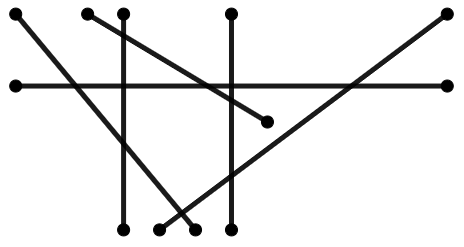
\includegraphics[width=9cm]{Imagenes/Ej3-P3-IO2021.PNG}
    %\caption{Ejemplo con 7 segmentos}
\end{figure}
 
\end{quest}

%%% TERMINA EL EJERCICIO 3 %%%

%%% EMPIEZA EL EJERCICIO 4 %%%


\begin{quest} 
Un grafo se dice ``de intervalos" si es el grafo intersección de intervalos abiertos en la recta real, es decir, si se pueden representar sus vértices a través de intervalos abiertos de modo de que cada intervalo está asociado a un vértice y dos vertices son adyacentes si y solo si los intervalos se intersecan. Por ejemplo el grafo:

\begin{center}
    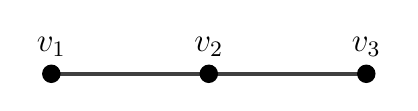
\begin{tikzpicture}
            \SetVertexStyle[FillColor=black, MinSize=0.7]
            \Vertex[label=$v_1$, position=above, fontsize=\large, x=0, y=0]{s1}
            \Vertex[label=$v_2$, position=above, fontsize=\large, x=2, y=0]{s2}
            \Vertex[label=$v_3$, position=above, fontsize=\large, x=4, y=0]{s3}
            \Edge(s1)(s2)
            \Edge(s2)(s3)
    \end{tikzpicture}
\end{center}

es de intervalos porque tiene, entre otras, la siguiente representación en intervalos:

\begin{center}
    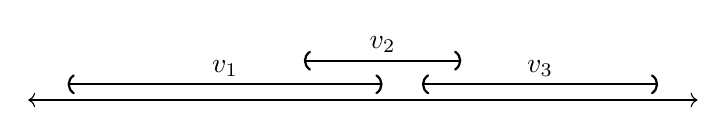
\begin{tikzpicture}
            \draw[<->] (0,0) -- (8.5,0);
            \draw[(-), thick] (0.5,0.2) -- (4.5,0.2);
            \node (v1) at (2.5, 0.4) {$v_1$};
            
            \draw[(-), thick] (3.5,0.5) -- (5.5,0.5);
            \node (v1) at (4.5, 0.7) {$v_2$};
            
            \draw[(-), thick] (5,0.2) -- (8,0.2);
            \node (v1) at (6.5, 0.4) {$v_3$};
            
    \end{tikzpicture}
\end{center}

\begin{enumerate}[(a)]
    \item Mostrar un grafo que no sea de intervalos. Justificar.
    
    \item Un grafo de intervalos es de intervalos unitario, si existe una representación de modo que todos los intervalos tengan la misma longitud. 
    Mostrar un grafo de intervalos que \textbf{no} sea de intervalos unitarios. Justificar.
\end{enumerate}

\end{quest}

%%% TERMINA EL EJERCICIO 4 %%%

%%% EMPIEZA EL EJERCICIO 5 %%%

\begin{quest}

Una empresa que sintetiza químicos debe transportar por medio terrestre su producción desde la planta ubicada en la ciudad $p_1$ hasta la ciudad $p_n$. No hay una ruta que conecte directamente a ambas ciudades, sino que hay caminos que pasan por ciudades intermedias $p_2, \dots, p_n$. 
%Por la naturaleza del producto, cada vez que se arriba a una ciudad, se debe cambiar el camión donde es transportado. Además, 
Al tratarse de una carga peligrosa, para $2\leq i\leq n-1$, la ciudad $p_i$ cobra un impuesto de $c_i$ pesos por unidad y no permite que pasen más de $r_i$ unidades mensuales.

Por otro lado, si existe un ruta directa desde $p_i$ a $p_j$ ($1\leq i,j\leq n$), la logística de la empresa puede transportar a lo largo de ella a lo sumo $q_{ij}$ unidades mensuales; el costo de transporte por unidad es de $s_{ij}$ pesos.

El objetivo de la empresa es maximizar la cantidad mensual de producción que puede transportar desde $p_1$ a $p_n$ minimizando los costos que implican la logística y los impuestos. Modelar como un problema de grafos y proponer un algoritmo que resuelva el problema en tiempo polinomial.


% Una empresa de turismo se encarga de organizar viajes terrestres desde la ciudad $p_1$, capital del país, hasta la ciudad $p_n$, que es otro destino turístico muy importante. No hay una ruta directa que conecte a $p_1$ con $p_n$, sino que hay distintos caminos que pasan por pueblos pintorescos $p_2,\dots,p_{n-1}$ que también son atractivos para los viajantes. Por lo tanto, la idea de la empresa es que si un turista pasa por cierto pueblo $p_i$ (con $2\leq i\leq n-1$), se hospede una noche allí antes de continuar su viaje. Para $2\leq i\leq n-1$, el precio unitario de hospedaje de un turista en el pueblo $p_i$ es $c_i$ y la capacidad hotelera es $r_i$.

% Por otro lado, si existe una ruta directa desde $p_i$ a $p_j$, la capacidad de transporte de la empresa viene dada por $t_{ij}$ y el costo unitario de transporte por turista viene dado por $\ell_{ij}$.

% El objetivo de la empresa es maximizar la cantidad de turistas desde $p_1$ hasta $p_n$ minimizando los costos que implican el hospedaje y el transporte. Modelar como un problema de flujo y proponer un algoritmo que resuelva el problema en tiempo polinomial.
    

\end{quest}

%%% TERMINA EL EJERCICIO 4 %%%

%%% TERMINA EL PARCIAL %%%



\end{document}

